\documentclass[12pt]{article}
\usepackage[a4paper, hmargin=1.25in,vmargin=1in]{geometry}
\usepackage{amsmath}
\usepackage{amssymb}
\usepackage{wasysym}
\usepackage{CJKutf8}
\usepackage{ulem}
%\usepackage[normalem]{ulem}
\usepackage{textcomp}
\usepackage{siunitx}
\usepackage{lettrine}
\usepackage{indentfirst} %強制首段縮排
\usepackage{xcolor}
\usepackage{graphicx} % 插入圖片用(p50)
\usepackage{fancyvrb} % 程式碼區塊
%帶行號的程式碼區塊
\usepackage{multicol} % 多欄
\usepackage{hyperref} %容易衝突,要放最後 p.37
\hypersetup{
	colorlinks=true,
	linkcolor=teal,%blue,
	filecolor=violet,%magenta,      
	urlcolor=cyan,
	pdftitle={Overleaf Example},
	pdfpagemode=FullScreen,
}
\setlength{\parindent}{1em} %水平長度(縮排)
\setlength{\parskip}{2pt plus 2pt minus 2pt} %垂直長度

\newenvironment{tightcenter}{%
	\setlength\topsep{0pt}
	\setlength\parskip{0pt}
	\begin{center}
	}{%
	\end{center}
}

\newenvironment{tightright}{%
	\setlength\topsep{0pt}
	\setlength\parskip{0pt}
	\begin{flushright}
	}{%
	\end{flushright}
}

\newenvironment{tightleft}{%
	\setlength\topsep{0pt}
	\setlength\parskip{0pt}
	\begin{flushleft}
	}{%
	\end{flushleft}
}

\title{The Title\thanks{ha ha ha}}
\author{OU, KAI-HAO\\CSIE\thanks{cmlab}, NTU}
\date{October 10, 2021}

% \renewcommand{\thesection}{Section.~\arabic{section}} % 詳見p.47
% \renewcommand{\thesection}{\arabic{section}.} % 詳見p.47

\begin{document}
%\begin{CJK*}{UTF8}{bsmi} %細明體
\begin{CJK*}{UTF8}{bkai} %標楷體	
	\maketitle
	\tableofcontents
	\begin{abstract}
	把摘要輕鬆帶過,顯然並不適合。摘要對我來說有著舉足輕重的地位,必須要嚴肅認真的看待。在人類的歷史中,我們總是盡了一切努力想搞懂摘要。
	\end{abstract}
	
	\newpage
	\section{大綱}
	
	這裡是大綱,也可輸入英文 \\
	You can also type english here.
	
	\LaTeX
	
	\LaTeXe
	
	\TeX
	
	測試! Hello world!
	
	\section{先備知識}
	
	查看 macro 的文檔:\\	
	[例如] texdoc ctex \\
	
	\noindent手寫符號辨識:Detexify \\ 
	https://detexify.kirelabs.org/classify.html \\
	
	\noindent公式截圖識別:Snip \\ 
	https://mathpix.com/ \\
	
	\section{CH3 latex基礎}
	
	$\backslash$  \\
	\textbackslash  \\
	\texttt{\char92}  \\
	\texttt{\char`\\}  \\
	\texttt{\char`~}  \\
	\texttt{\char`@}  \\
		
	\mbox{}\\
	a $\sim$ b  \\
	a\textasciitilde b  \\
	a\~{}b  \\
	a\~b  \\
	
	\mbox{}\\
	$>$ \\
	$<$ \\
	\textgreater \\
	\textless \\
	
	\mbox{}\\	
	`` `Max' is here.''。\\
	``\thinspace`Max' is here.''。\\
	
	\mbox{}\\	
	KAI-HAO\\
	page 1--2\\
	Listen---I'm serious.\\	
	中文省略號......\\
	英文省略號$\ldots$\\
	
	\noindent斜體表強調 \emph{gg gg gg} (斜體文本中,「正體」表強調) \\

	\mbox{}\\
	\uline{底線} \\
	\uuline{雙底線} \\
	\uwave{波浪線} \\
	\sout{刪除線} \\
	\xout{斜刪除線} \\
	\dashuline{虛 底線} \\
	\dotuline{點 底線} \\
	\uline{底\uuline{雙\xout{斜刪除線}底線}線} \\
	\emph{gg g\emph{gg gg gg}g gg} \\
	
	\mbox{}\\	
	\ang{30.33} \\
	$30^{\circ}\mathrm{C}C$ \\
	$30\,^{\circ}\mathrm{C}C$ \\
	$30\,$\textcelsius \\
	
	\mbox{}\\	
	歐元:\texteuro \\
	\mbox{1\,000\,000}\textdollar \\
	\mbox{1000\textperthousand} \\
	\mbox{\num[group-separator={,}]{1234567890}\textdollar}
	
	\begin{tightright}
	\=o
	\^o
	\d{o}
	$\tilde{o}$
	\o
	\aa
	\oe
	\'o
	\"o
	\u{o}
	\O
	\AA
	\OE
	\v o
	\.o
	\b{o}
	$\hat{o}$
	\i
	\ae
	!`
	\`o
	\H{o}
	\t{oo}
	\j
	\AE
	?`
	\end{tightright}
	
	\mbox{}		
	
	\begin{tightcenter}
	防止換行用\textasciitilde\\	
	防止換行用\textasciitilde\\
	如Fig.~99 %p27	
	\end{tightcenter}	
	
	Page 100,  Page 100,  Page 100,  Page 100,  Page 100,  Page 100,  Page 100,  Page 100,  Page 100,  Page 100,  Page 100.
	
	Page~100,  Page~100,  Page~100,  Page~100,  Page~100,  Page~100,  Page~100,  Page~100,  Page~100,  Page~100,  Page~100.
	
	電話號碼不想被斷詞 \mbox{+886 912 778 955} % p67
	
	\mbox{}
	
	\centerline{center text without adding space}
	
	\mbox{}
	
	帶有縮排的新段:段落文字文字,段落文字文字,段落文字文字,段落文字文字,段落文字文字。
	帶有縮排的新段:段落文字文字,段落文字文字,段落文字文字,段落文字文字,段落文字文字。
	\par帶有縮排的新段:段落文字文字,段落文字文字,段落文字文字,段落文字文字,段落文字文字。
	
	\mbox{}
	
	\lettrine{首字}{放大}的效果的效果的效果的效果的效果的效果的效果的效果的效果的效果的效果的效果的效果的效果的效果,的效果的效果的效果的效果的效果的效果的效果的效果的效果的效果的效果的效果。
	
	\mbox{}\\
	無襯線 \sffamily{sans-serif}\\
	等寬字 \ttfamily{Hello!}\\
	羅馬字 \rmfamily{Roman}\\	
	{\mdseries{中a8}粗Regular}\\
	{\bfseries{粗a8}體Bold}\\
	小號大寫體 \scshape{Caps and Small Caps}\\
	強調 \itshape{italic}\\
	斜 \slshape{slanted}\\
	直 \upshape{upright}\\
	
%	\tiny
%	\scriptsize
%	\footnotesize
%	\small
%	\normalsize (default)
%	\large
%	\Large
%	\LARGE
%	\huge
%	\Huge
	
	% inline
	{\fontsize{22}{\baselineskip}\selectfont Text Size Demo.\\}
	{\fontsize{23}{\baselineskip}\selectfont Text Size Demo.\\}
	{\fontsize{24}{\baselineskip}\selectfont Text Size Demo.\\}
	{\fontsize{50}{60}\selectfont Foo}
	{\fontsize{5}{6}\selectfont bar!}
	{\Huge Foo}
	{\tiny bar!}
	{\Large This is some large text\par}
	% environment
	\begin{footnotesize}
		text size environment...
	\end{footnotesize}

	Let's change font to {\fontfamily{lmss}\selectfont Palatino} % p.32 表3.5
	
	\noindent\mbox{}\\
	文字顏色:\\
	{\textcolor{pink}{TXT:pink.}} \\
	{\textcolor{red}{TXT:red.}} \\
	{\textcolor{orange}{TXT:orange.}} \\
	{\textcolor{yellow}{TXT:yellow.}} \\
	{\textcolor{lime}{TXT:lime.}} \\
	{\textcolor{green}{TXT:green.}} \\
	{\textcolor{olive}{TXT:olive.}} \\
	{\textcolor{teal}{TXT:teal.}} \\
	{\textcolor{cyan}{TXT:cyan.}} \\
	{\textcolor{blue}{TXT:blue.}} \\
	{\textcolor{violet}{TXT:violet.}} \\
	{\textcolor{purple}{TXT:purple.}} \\
	{\textcolor{magenta}{TXT:magenta.}} \\
	{\textcolor{brown}{TXT:brown.}} \\
	{\textcolor{white}{TXT:white.}} \textless- white\\
	{\textcolor{lightgray}{TXT:lightgray.}} \\
	{\textcolor{gray}{TXT:gray.}} \\
	{\textcolor{darkgray}{TXT:darkgray.}} \\
	{\textcolor{black}{TXT:black.}} \\
	\mbox{}\\
	{\textcolor{red!70}{70\%紅色}} \\
	{\textcolor{-yellow}{黃色的互補色}} \\

	\subsection{CH3-5 引用與註釋 (p.37)}

	% chapter section figure table equation code listing

	\label{figure:test}	
	See figure~\ref{figure:test} on page~\pageref{figure:test}.
	
	\label{section:XXX}
	See section~\ref{section:XXX} on page~\pageref{section:XXX}.

	we have solved equation \eqref{eq:QQQ} %\ref{eq:QQQ} 
	
	
	\mbox{}\\
	{\Large Hyperref} \\	
	\hyperref[section:XXX]{GO TO section:XXX}\\
	The equation \ref{eq:QQQ} shows in the page \pageref{eq:QQQ}.\\	
	HyperLink:  \href{http://www.overleaf.com}{Something Linky}\\
	 or go to the next url: \url{http://www.overleaf.com}\\
	 or open the next file \href{run:./file.txt}{File.txt}\\
	 
	幫我來個註腳\footnote{這是個註腳。}\\
	
	來個邊註\marginpar[左左]{右右}\\

	\begin{quote}
		引用文字,引用文字;\\
		引用文字,引用文字。
		
		引用文字,引用文字;\\
		引用文字,引用文字。
	\end{quote}
	
	\begin{quotation}
		引用文字,引用文字;\\
		引用文字,引用文字。
		
		引用文字,引用文字;\\
		引用文字,引用文字。
	\end{quotation}

	\begin{itemize}
		\item 第一項
			\begin{itemize}
			\item[-] 第二項
			\item[*] 第二項
			\item[+] 第二項
			\end{itemize}
	\end{itemize}
	\mbox{}\\
	\begin{enumerate}
		\item AAA
		\item[斷啦!] BBB
		\item CCC
	\end{enumerate}
	\mbox{}\\
	\begin{description}
	\item This is an entry \textit{without} a label.
	\item[變粗!] A short one-line description.
	\item[變粗?] A much longer description.
	\end{description}

	%插入圖片
	\graphicspath{{./fig/}{./}} %圖片搜尋路徑
	
	\begin{center}
		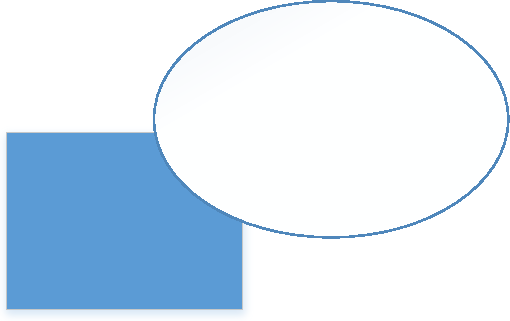
\includegraphics[width=0.3\linewidth]{p1.pdf}
	\end{center}

	%浮動體 圖片
	\begin{figure}[!htb]
		\centering
		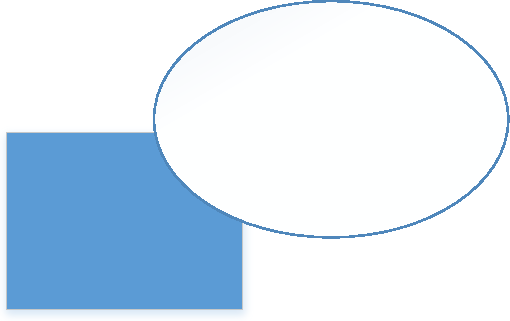
\includegraphics[width=0.3\linewidth]{p1.pdf}
		\caption{範例圖片的標題}
		\label{fig:FFFFF}		
	\end{figure}
	
	%浮動體 表格
	\begin{table}[!htb]
		\centering
		\caption{範例表格的標題}
		\label{table:TTTTT}	
		\begin{tabular}{ c c c }
			cell1 & cell2 & cell3 \\ 
			cell4 & cell5 & cell6
		\end{tabular}	
	\end{table}

	\begin{center}
		\begin{tabular}[c]{| l | c || p{3em} ||| r | @{**}  }
			\hline\hline
			
			AA & BB & CC & dd\\
			
			D & E & F & g\\
			
			\cline{1-2}
			
			\multicolumn{2}{|c|}{G}  &  H  &  i \\
			
			\hline
		\end{tabular}
	\end{center}

	\noindent\\
	\verb|#include<iostream>|\\
	\verb|int main(void){ }|\\
	\verb*|int main(void){ }|
	
	\begin{verbatim}
		#include<iostream>
		int main(void){ }
	\end{verbatim}

	\begin{verbatim*}
	#include<iostream>
	int main(void){ 
		}
	\end{verbatim*}

	\begin{Verbatim}
1234567890
	12345678901234567890
		1234567890
	12345678901234567890
1234567890
	\end{Verbatim}
	
	\begin{Verbatim}[tabsize=4]
	1234567890
		12345678901234567890
			1234567890
		12345678901234567890
	1234567890
	\end{Verbatim}

	\begin{multicols}{3}
	[\subsection{Multicols}The text placed here can be displayed in a cross-column representation. This is really convenient when writing abstract layouts!]
	Two-column documents can be easily created by passing the parameter \verb|\twocolumn| to the document class statement. If you need more flexibility in the column layout, or to create a document with multiple columns, the package \verb|multicol| provides a set of commands for that.	% \columnbreak
	\end{multicols}

	\mbox{}\\ %p68
	OK. That's fine.\\
	OK\@. That's fine.\\
	OK.\@ That's fine.\\
	Prof. OU is a nice man.\\
	Prof.~OU is a nice man.\\ %不允許斷行
	Prof.\ OU is a nice man.\\ %允許斷行

	\mbox{}\\
	\permil \\
	\hexstar \\
	\male \\
	\female \\
	\XBox \\
	\checked \\
	\CheckedBox \\
	\phone \\
	\twonotes \\




	\newpage
	\section{CH4 latex數學排版}
	
	\begin{equation} \label{eq:QQQ}
		x^2 - 5 x + 6 = 0
	\end{equation}

	${A^{\dagger}}$
		
	$\begin{pmatrix} 
		\text{氣溫}_1 & \text{氣溫}_n \\
		\text{濕度}_1 & \text{濕度}_n 
	\end{pmatrix}$\par

	
	\newpage\mbox{}\newpage\mbox{}\newpage
	
	an article~\cite{RN42}
	
	\bibliographystyle{plain} % Choose style for bibliography (選擇引文的格式)	{可選:prsty / abbrv / alpha / plain / unsrt}
	\bibliography{refxxx}        % ref.bib is the name of our database
	
\end{CJK*}
\end{document}